\section{Git}

Git, a distributed version control system, was created in 2005 by Linus
Torvalds, the Linux kernel's founder. This event occurred after a
\href{https://graphite.dev/blog/bitkeeper-linux-story-of-git-creation}{licensing
dispute with BitKeeper}, the previous versioning system used to maintain Linux.
-Torvalds, with contributions from other Linux developers, designed Git to
improve on the de-facto standard of the time that was Apache Subversion (SVN).
Specifically, Git was intended to be used in a decentralized manner, allowing
the user to work offline by copying the entirety of the change history when
first cloning a repository. Additionally, Git introduced better tools for
handling merge conflicts when multiple contributors wanted to modify the same
sources. These features proved to be indispensable for larger open-source
projects. Today, SVNs are rarely heard of anymore while Git is the de-facto
industry standard.

Today, we are going to focus on working with the command line tool \textbf{git}.
This tool allows its user to manage the versioning of a project locally and
optionally, to sync the changes with a remote repository stored on platforms
such as \href{https://github.com/}{GitHub} or
\href{https://about.gitlab.com/}{GitLab}. We recommend creating an account on
the former if you don't already have one. This will come in handy when you will
be asked to create your first repository and push a number of changes later on
in the practical part of this session. Note however that an account is not
required in order to clone public projects on your local machine. Moving
forward, we recommend that you clone a repository in order to  explore some of
the features of the \textbf{git} tool. Large repositories such as the
\href{https://github.com/torvalds/linux}{Linux kernel} have a long history (of
over 1.3 million commits in this case) that will result in upwards of 5GB of
downloaded data. Try finding a smaller repository that can be more manageable.
For example, \href{https://github.com/LizardByte/Sunshine}{Sunshine}.

\begin{lstlisting}[style=bashstyle]
$ sudo apt install -y git
$ git clone https://github.com/LizardByte/Sunshine.git
$ cd Sunshine/
\end{lstlisting}

\subsection{Commits}

A Git commit is a snapshot of changes made to the files in a Git repository at
a specific point in time. The current form of the data in the repository is a
result of iteratively applying these patches on top of one another. This is
the reason why cloning well-known projects with many contributions takes time.
Alternatively, you can create a \textit{shallow clone} by specifying the
\texttt{--depth} flag which will truncate the history to a specific number of
commits. On the one hand, this will reduce the amount of information downloaded
and will spare computation resources that would otherwise be wasted on computing
the latest version of each file. On the other hand, a shallow clone will not
permit you to investigate the history of a project if you need to identify the
exact moment when a bug was introduced.

\begin{figure}[h]
    \centering
    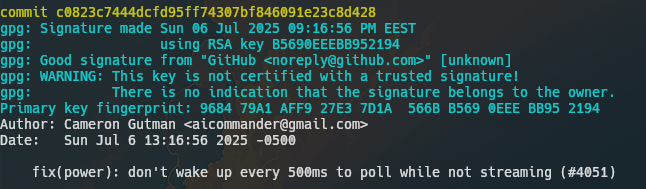
\includegraphics[width=\textwidth,keepaspectratio]{figures/git-log-good.png}
    \caption{One commit in the git log of a repository.}
    \label{fig:git-log}
\end{figure}

When looking at the \textbf{git log} of a repository, you will see a sequence of
entries such as that in Figure \ref{fig:git-log}. Each commit is identified via
a 40-character long \textbf{hexstring}. A hexstring is the hexadecimal
representation of a sequence of bytes, where every nibble (i.e., 4 bits) is
represented by a character ranging from \textit{'0' (= 0b0000)} to \textit{'F'
(= 0b1111)}. But how is this identifier calculated?

This commit identifier is called a hash value or a digest, and is the output of
a \href{https://en.wikipedia.org/wiki/Hash_function}{hash function}. A hash
function takes an arbitrary amount of data and outputs a fixed-size bit array
that is representative of the input. Normally, one would be weary of collisions:
if the function's domain is virtually infinite and the co-domain is not only
finite but rather small in comparison, wouldn't it be possible to create two
commits with the same digest? Possible - yes, likely - no. Git uses SHA1, a
\href{https://en.wikipedia.org/wiki/Cryptographic_hash_function}{cryptographic
hash function}. What makes a cryptographic hash function so special is that it
provides certain guarantees. For example, it should be impossible to calculate
potential messages from a digest (meaning that the function is non-invertible).
Moreover, any change in the input - no matter how small, should change the hash
value so extensively that the new value and the old should appear uncorrelated.
Consequently, being able to craft a commit such that it's not only
comprehensible, but also creates a certain desired digest is so unlikely that it
occurring naturally should not pose any risk. These concepts will be explored in
more detail later on, in the Security Fundamentals lesson of this module.

There is, however, a more significant risk here. What guarantee do you have that
the author of the commit above is actually who he says he is? Using something
like \href{https://github.com/jayphelps/git-blame-someone-else}
{git-blame-someone-else}, you could overwrite commits and change their author
only to then \texttt{git push --force} and replace the remote history (don't do
this on the master branch if you're not working alone). The answer to this
problem is commit signing. Cryptographic algorithms can be loosely categorized
as symmetric and asymmetric. Symmetric algorithms such as
\href{https://en.wikipedia.org/wiki/Advanced_Encryption_Standard}{AES} use the
same key for both encryption and decryption. Asymmetric algorithms such as
\href{https://en.wikipedia.org/wiki/RSA_cryptosystem}{RSA}, on the other hand,
utilize two keys. One for encryption and one for decryption. Usually, the one
used for encryption is called the private key and the one used for decryption,
the public key. The private key is your identity, so you don't share it with
anyone. The public key you configure on remote servers to give them the ability
to verify your identity (e.g.: configuring SSH keys on a server). As a rule, you
use asymmetric cryptography in cases where you need to prove your identity to a
remote host, establish secure communication channels over an untrusted network,
etc. The reason for this is that asymmetric algorithms are orders of magnitude
slower than their symmetric counterparts. While encrypting the output of a
SHA256 function (32 bytes) with a 4096-bit RSA key takes about 5ms on regular
CPUs, it takes almost a full minute on an Arduino Mega (with a MCU running at
16MHz). AES-256 on the other hand, encrypts the same amount of data in less than
5 microseconds. The downside is that you need to share your key with other
systems for them to extract the plaintext message.

\begin{figure}[h]
    \centering
    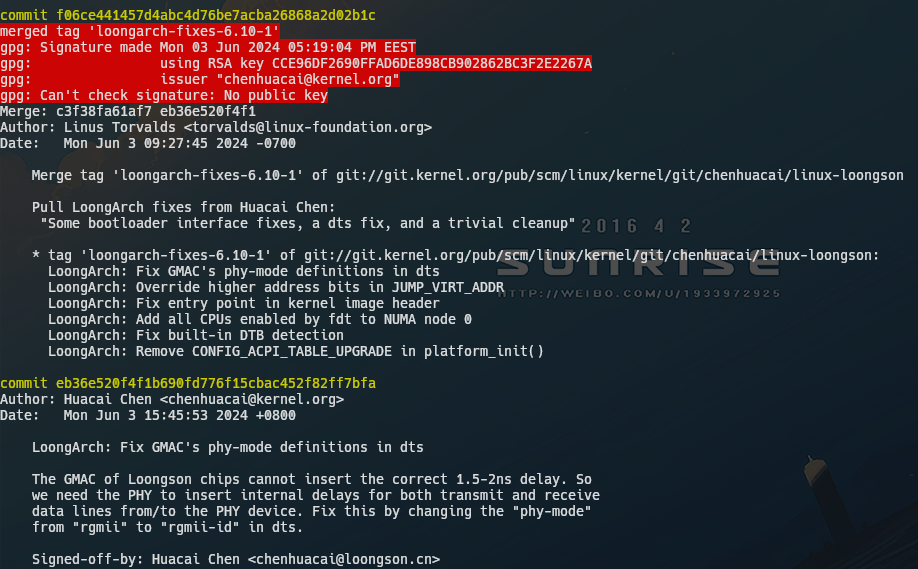
\includegraphics[width=\textwidth,keepaspectratio]{figures/git-log-bad.png}
    \caption{Git commits that have either an unverified signature, or no
             signature at all.}
    \label{fig:git-log-bad}
\end{figure}

In Figure \ref{fig:git-log} you can identify the \textbf{Author} of the
commit and the \textbf{Date} when the commit was created. However, there is an
additional output from \textbf{GNU Privacy Guard (GPG)}. This output was
generated because the \textbf{--show-signature} flag was used when viewing the
commit log. As a result, \textbf{git} deferred to \textbf{gpg} for verifying the
authenticity of each commit that was signed. In this case, the commit was not
signed by the author, but as a result of automatic processing of contributions
(i.e., pull requests) or edits created directly in the web interface (less
likely in this situation). In Figure \ref{fig:git-log-bad} we can see two
additional examples where one commit's signature could not be verified and
another's is missing. The reason why the first signature could be verified is
that we used the \texttt{gpg --search-keys} feature to look up a public key in
public key servers based on their fingerprint or the email address of the
owner. However, the authenticity of the key associated to
\texttt{noreply@github.com} was not guaranteed by a trusted third party. As a
result, it was included in our \href{https://www.gnupg.org/gph/en/manual/c235.html}
{GPG keyring} but with a limited level of trust, which shouls in the
\texttt{git log} annotation.

\subsection{Choosing a license}

If you ever decide to publish code that you've written, note that it will
automatically fall under the protection of copyright law. This means that
distributing copies of your code, or using it as a basis for something that may
be construed as derivative work is prohibited. As a result, people will
generally stay clear of your project since they don't know what your intentions
are.

In the 1980s, \href{https://www.youtube.com/watch?v=jUibaPTXSHk}{Richard
Stallman} pioneered concepts known today as \textbf{free software} and
\textbf{copyleft}. Free software is software distributed with a guarantee that
the end user can modify and adapt it for whatever purpose, profit included. In
order for this to happen, the user must have ultimate control over the software
in question, which implies access to the source code. So, for a piece of
software to become "free software" it must include a public license such as the
GNU General Public License, MIT license, etc. These licenses waive part of the
author's rights and and grants them to the recipient of the software. Almost all
free-software licenses contain a copyleft provision. This provision states that
when modified versions of the free software are distributed, it must provide
the same guarantees as the original, under the same license (or a more
permissive one).

Note that certain projects such as third-party libraries are sometimes published
under a dual license. One of them may require the recipient to open source their
code (that uses said library) but the other may grant them the possibility of
\textit{not} publishing their code in exchange for purchasing a license. This is
a requirement even if the library is linked as a shared library, and not
compiled statically as part of the distributed binary. Nonetheless, certain
parties have made the argument that writing a wrapper application over the
thrid-party library and using an Inter-Process Communication (IPC) mechanism
to interact with it \textit{could} restrict the applicability of the library's
license only to the wrapper itself and not to the main application as well.
It is good to know that such discussions exist but we do not advise to use this
approach for several reasons, most notably that a) it goes against the ethos of
the free, open-souce software movement and b) it is unclear if this reasoning
can be upheld in legal court.

If you want to learn more about different kinds of licenses (or licenses in
general), listen to this episode of the
\href{https://www.youtube.com/watch?v=dsm1SKqVsTQ&t=406s}{Destination Linux
podcast}.
